\documentclass[10pt]{article}
\usepackage{pgfplots}
\pgfplotsset{compat=1.15}
\begin{document}
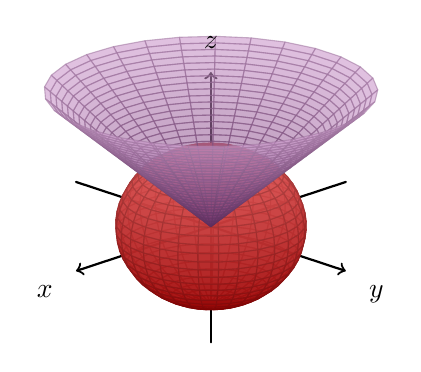
\begin{tikzpicture}[line cap=round, line join=round]
\begin{axis}[
    view={135}{25}, % Rotamos la cámara: x a la izquierda, y a la derecha
    axis lines=center,
    xmin=-4, xmax=4,
    ymin=-4, ymax=4,
    zmin=-3, zmax=4,
    ticks=none,
    axis line style={thick, ->},
    xlabel={$x$},
    ylabel={$y$},
    zlabel={$z$},
    % Forzamos la posición de las etiquetas a la punta de los ejes
    every axis x label/.style={at={(ticklabel* cs:1.05)},anchor=north east},
    every axis y label/.style={at={(ticklabel* cs:1.05)},anchor=north west},
    every axis z label/.style={at={(ticklabel* cs:1.05)},anchor=south},
]

% Esfera roja (radio 2)
\addplot3[
    surf,
    opacity=0.8,
    colormap={redmap}{color=(red!60!black) color=(red!50!white)},
    samples=30,
    domain=0:360,
    y domain=0:180,
    z buffer=sort
]
({2*cos(x)*sin(y)}, {2*sin(x)*sin(y)}, {2*cos(y)});

% Cono violeta (z = sqrt(x^2 + y^2))
\addplot3[
    surf,
    opacity=0.6,
    colormap={purplemap}{color=(violet!50!black) color=(violet!40!white)},
    samples=30,
    domain=0:360,
    y domain=0:3.5,
    z buffer=sort
]
({y*cos(x)}, {y*sin(x)}, {y});

\end{axis}
\end{tikzpicture}
\end{document}

